\documentclass[conference]{IEEEtran}
\IEEEoverridecommandlockouts

% Packages
\usepackage{cite}
\usepackage{amsmath,amssymb,amsfonts}
\usepackage{algorithmic}
\usepackage{graphicx}
\usepackage{textcomp}
\usepackage{xcolor}

\def\BibTeX{{\rm B\kern-.05em{\sc i\kern-.025em b}\kern-.08em
T\kern-.1667em\lower.7ex\hbox{E}\kern-.125emX}}

\begin{document}

\title{Agentic AI for Real-Time Air Quality Prediction\\
and Autonomous Environmental Response}


\author{

\IEEEauthorblockN{Muhammad Saad Khalid Khan Suri}
\IEEEauthorblockA{
\textit{Department of Computer Science}\\
\textit{University of Engineering and Technology}\\
Lahore, Pakistan\\
2025mscs238@student.uet.edu.pk
}
\and
\IEEEauthorblockN{Abqa Javed}
\IEEEauthorblockA{
\textit{Department of Computer Science}\\
\textit{University of Engineering and Technology}\\
Lahore, Pakistan\\
abqa.javed@uet.edu.pk
}

\IEEEauthorblockA{\hspace{7cm}} % Creates a new row

\IEEEauthorblockN{Aatif Hussain}
\IEEEauthorblockA{
\textit{Department of Computer Science}\\
\textit{University of Engineering and Technology}\\
Lahore, Pakistan\\
aatif@uet.edu.pk
}
\and
\IEEEauthorblockN{Abdul Ahad Khan Suri}
\IEEEauthorblockA{
\textit{Department of Computer Science}\\
\textit{The University of Lahore}\\
Lahore, Pakistan\\
70131507@student.uol.edu.pk
}


}
\maketitle


\begin{abstract}
Rapid urbanization and industrial growth have exacerbated air pollution, presenting a critical threat to global public health. While traditional environmental monitoring systems provide passive data visualization, they fail to deliver proactive, autonomous interventions. This paper presents a novel, production-ready platform that integrates real-time Air Quality Index (AQI) prediction with a multi-agent Artificial Intelligence (AI) framework. Utilizing an Extreme Gradient Boosting (XGBoost) model trained on high-resolution meteorological and pollutant data, the system achieves an $R^2$ score of 0.9929 and a Mean Absolute Error (MAE) of 0.85 in AQI forecasting. Furthermore, a Large Language Model (LLM)-powered multi-agent architecture evaluates these predictions to autonomously dispatch contextual alerts and mitigation strategies. The system is containerized via Docker and features a high-performance FastAPI backend coupled with a real-time Streamlit dashboard. Experimental results demonstrate the efficacy of combining predictive machine learning with agentic decision-making to transition smart cities from passive monitoring to active environmental management.
\end{abstract}

\begin{IEEEkeywords}
Air Quality Index (AQI), Agentic AI, Machine Learning, XGBoost, Smart Cities, Internet of Things (IoT), Multi-Agent Systems.
\end{IEEEkeywords}

\section{Introduction}

Air pollution remains one of the most pressing environmental challenges affecting both developed and developing countries. Rapid industrialization, urban expansion, increasing vehicular emissions, and energy consumption have significantly contributed to the deterioration of air quality.Air pollution remains one of the most pressing environmental challenges affecting both developed and developing countries \cite{b8,b9}. Rapid industrialization, urban expansion, increasing vehicular emissions, and fossil-fuel-based energy consumption have significantly contributed to the deterioration of air quality \cite{b10,b11}. Exposure to elevated concentrations of airborne pollutants has been associated with respiratory diseases, cardiovascular disorders, reduced life expectancy, and substantial economic losses \cite{b12,b13}. Consequently, continuous air quality monitoring and timely intervention have become essential components of sustainable urban development and public health protection.

Recent advances in the Internet of Things (IoT) have enabled the deployment of distributed sensor networks capable of collecting environmental data at high temporal resolution \cite{b14,b15}. These sensors continuously measure pollutant concentrations, meteorological conditions, and atmospheric parameters, providing valuable information for environmental monitoring. However, the majority of existing monitoring systems function primarily as data collection and visualization platforms. They present historical or real-time measurements to users but rely heavily on manual interpretation before any preventive or corrective actions can be taken.

Machine Learning (ML) has emerged as an effective solution for forecasting Air Quality Index (AQI) valuesMachine Learning (ML) has emerged as an effective solution for forecasting Air Quality Index (AQI) values by learning complex nonlinear relationships between pollutant concentrations and meteorological variables \cite{b1,b2,b5,b6}. Ensemble learning techniques, particularly Extreme Gradient Boosting (XGBoost), have demonstrated high predictive accuracy while maintaining computational efficiency for structured environmental datasets. Despite these advances, most predictive systems terminate after generating AQI forecasts and do not provide intelligent decision support or automated environmental responses.

The emergence of Large Language Models (LLMs) and agent-based Artificial Intelligence offers new opportunities for autonomous reasoning and intelligent decision support \cite{b3,b4,b16,b17}. Unlike conventional AI applications that generate predictions alone, agentic AI systems are capable of reasoning over incoming data, coordinating specialized software agents, and producing context-aware recommendations without continuous human supervision. Such systems can transform environmental monitoring from a reactive process into a proactive framework capable of supporting public safety and smart city operations.

Motivated by these challenges, this research proposes an integrated Agentic AI framework for real-time air quality prediction and autonomous environmental response. The proposed architecture combines an XGBoost-based predictive model with a multi-agent reasoning framework powered by a Large Language Model. Real-time environmental data are processed through a FastAPI backend, while autonomous agents analyze predicted AQI values to generate health advisories, traffic management suggestions, and environmental mitigation recommendations. The entire platform is containerized using Docker and visualized through an interactive Streamlit dashboard, enabling scalable deployment for smart city applications  \cite{b16,b17,b25}.

The primary contributions of this research are summarized as follows:

\begin{itemize}
    \item Development of a highly accurate real-time AQI prediction model using the XGBoost algorithm.
    \item Integration of a multi-agent AI framework capable of autonomous reasoning and environmental decision-making.
    \item Design of a scalable cloud-ready architecture using FastAPI, Docker, and Streamlit for continuous environmental monitoring.
    \item Incorporation of explainable machine learning techniques to improve transparency and support trustworthy AI-driven environmental management.
\end{itemize}

\section{Literature Review}

Significant research has been conducted on AQI prediction utilizing various ML architectures. Early approaches relied on statistical models such as Autoregressive Integrated Moving Average (ARIMA) or Multiple Linear Regression (MLR). More recently, ensemble methods like Random Forest (RF) and Extreme Gradient Boosting (XGBoost) have demonstrated superior capacity in capturing the nonlinear dynamics between meteorological variables (wind speed, humidity) and pollutant dispersion. Concurrently, the advent of Large Language Models (LLMs) has spurred the development of multi-agent systems---networks of autonomous software agents capable of complex reasoning and task execution. While agents have been deployed in software engineering and financial modeling, their integration into continuous environmental IoT streams remains underexplored. Existing literature highlights a distinct gap: the lack of end-to-end frameworks that seamlessly fuse high-frequency ML inference with natural language-driven autonomous response mechanisms.

A granular examination of predictive \cite{b18,b19}. models reveals a clear dichotomy between classical statistical forecasting and modern machine learning. Autoregressive Integrated Moving Average (ARIMA) models are highly effective for univariate, linear time-series prediction where historical trend patterns remain stable. However, their primary weakness lies in their inability to process exogenous variables (e.g., sudden wind shifts and traffic spikes) or model the complex, nonlinear chemical interactions that govern atmospheric pollution. Conversely, Recurrent Neural Networks (RNNs) and Long Short-Term Memory (LSTM) networks excel in capturing long-term temporal dependencies in sequential data, making them robust for multi-step AQI forecasting. Nonetheless, LSTMs require substantial computational resources for training, exhibit relatively high inference latency, and function as ``black-box'' models, which limits their suitability for real-time edge-device deployment where explainability is essential \cite{b20,b21}.

Ensemble learning methods, such as Random Forest (RF) and XGBoost, offer a practical middle ground. RF reduces variance by averaging multiple uncorrelated decision trees, making it highly robust to noise and outliers in IoT sensor telemetry. However, it can be computationally expensive for high-frequency prediction tasks. XGBoost utilizes gradient boosting over regularized decision trees to optimize both computational speed and predictive accuracy. Its built-in handling of missing values and L1/L2 regularization minimizes overfitting while improving prediction accuracy. More recently, hybrid frameworks have emerged by combining LSTMs for temporal pattern extraction with tree-based models (e.g., LSTM-XGBoost) or residual correction layers. These hybrid systems achieve state-of-the-art performance by combining the temporal learning capability of neural networks with the precision of gradient-boosted decision trees, albeit at the cost of increased system complexity and deployment overhead \cite{b2,b5,b6,b22}.

\section{Proposed System Architecture}

\subsection{Problem Statement}

Current air quality monitoring platforms exhibit high latency between the detection of hazardous conditions and the dissemination of actionable mitigation strategies. Furthermore, deterministic alert thresholds lack the contextual awareness required for complex urban environments. Therefore, a dynamic, context-aware system is needed to autonomously synthesize sensor data, predict localized air quality degradation, and orchestrate intelligent responses without human-in-the-loop bottlenecks.

\subsection{Research Objectives}

This study aims to achieve the following objectives:

\begin{enumerate}
    \item Develop a highly accurate real-time AQI prediction pipeline using state-of-the-art ensemble regression models.
    \item Design a multi-agent AI framework capable of autonomous reasoning based on streaming environmental telemetry.
    \item Engineer a production-grade, containerized application stack that supports real-time data ingestion and visualization.
    \item Integrate Explainable Artificial Intelligence (XAI) techniques to improve model transparency and interpretability.
\end{enumerate}

\subsection{System Overview}

The proposed architecture comprises a hybrid pipeline consisting of a deterministic ML layer for quantitative AQI prediction followed by a stochastic LLM-based agent layer for qualitative reasoning. Data collected from IoT sensors undergoes immediate feature extraction before being processed by an XGBoost regressor to predict the AQI. The predicted AQI is subsequently categorized according to the United States Environmental Protection Agency (EPA) standards. When the predicted AQI exceeds predefined safety thresholds, the telemetry is forwarded to the Agentic AI framework. Using prompt chaining, the framework autonomously generates context-aware public health advisories, traffic management recommendations, and environmental mitigation strategies in real time.

\begin{figure*}[!t]
\centering
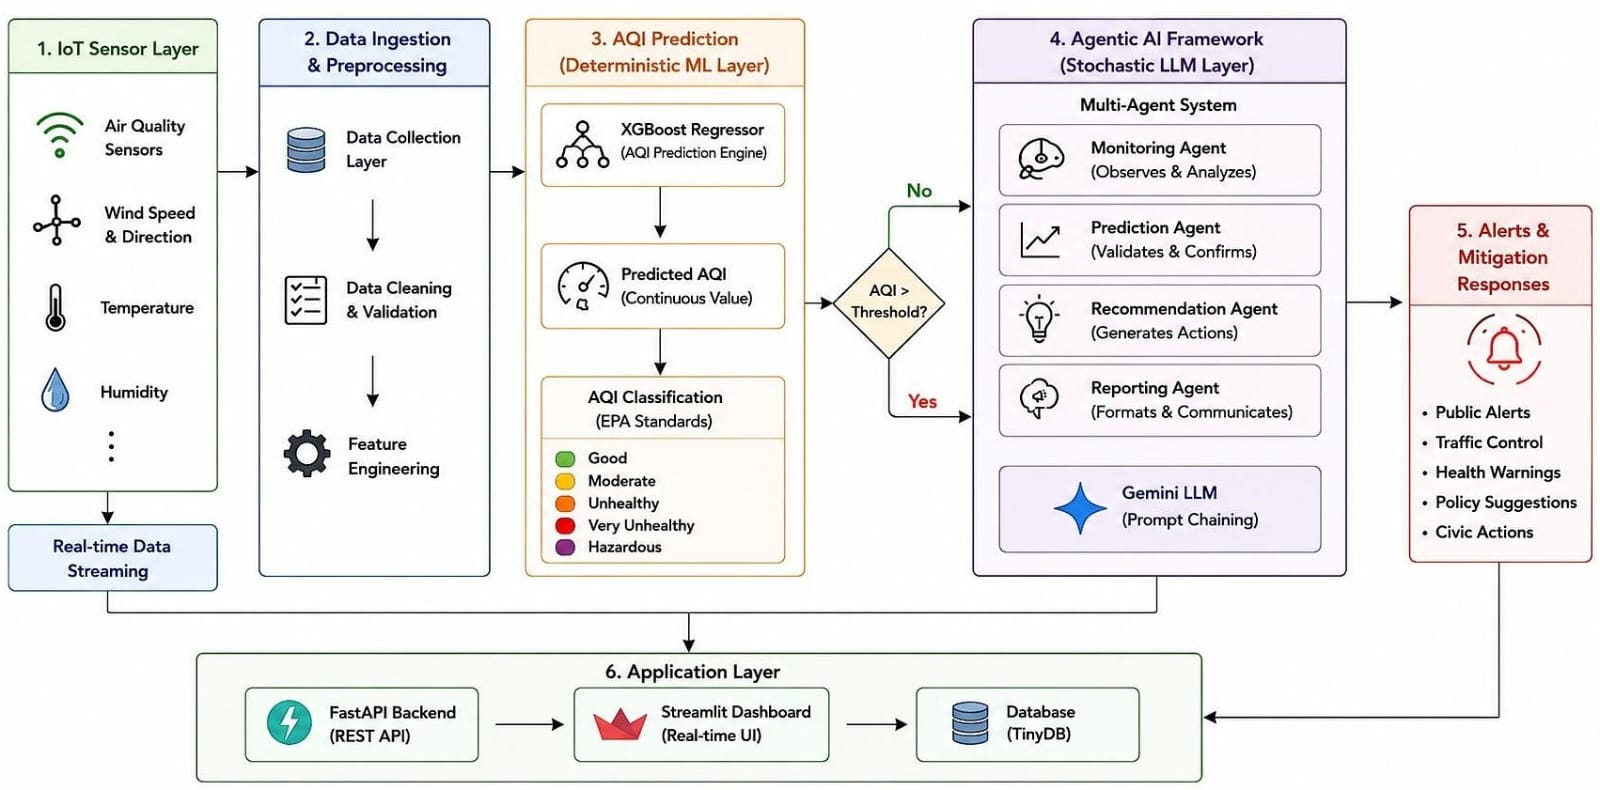
\includegraphics[width=\textwidth]{image1.jpeg}
\caption{System Architecture Diagram illustrating the hybrid pipeline: deterministic predictive ML layer (XGBoost) and multi-agent AI response orchestration layer (LangChain and Google Gemini).}
\label{fig:system_architecture}
\end{figure*}
\subsection{Data Collection and Dataset Design}

To facilitate robust model training and overcome the missing-data sparsity commonly encountered in public air quality APIs, a synthetic dataset containing 10,000 records was algorithmically generated.

The data generation process incorporated realistic environmental patterns, including diurnal traffic cycles, meteorological dispersion, and photochemical reactions. Rush-hour multipliers increased the concentrations of NO$_2$ and CO, while wind speed was inversely related to PM$_{2.5}$ and PM$_{10}$. Ozone (O$_3$) concentrations were modeled to peak during periods of maximum temperature. These mechanisms produced a diverse and representative dataset suitable for training and evaluating the proposed machine learning models.

\subsection{Data Preprocessing}

Preprocessing involved standardizing the numerical features and
splitting the dataset into training and validation sets using an
80:20 ratio. Since the selected models are tree-based,
additional feature scaling techniques, such as Min--Max
normalization, were unnecessary. This approach preserved the
original feature values while maintaining their interpretability.

\subsection{Feature Engineering}

Feature engineering focused on the six primary EPA criteria
pollutants. Temporal attributes, including timestamp indices,
were excluded from the final regression matrix to ensure that
the model relied solely on contemporary pollutant
measurements rather than memorizing temporal patterns. This
strategy minimized data leakage and improved the model's
generalization during real-time deployment.

\section{Predictive Modeling and Evaluation}

\subsection{Machine Learning Models}

The core predictive task was formulated as a multivariate
regression problem. Four machine learning models were
evaluated: Multiple Linear Regression (MLR) as the baseline,
Decision Tree Regressor (DTR) for capturing nonlinear
relationships, Random Forest (RF) for reducing variance, and
Extreme Gradient Boosting (XGBoost) for optimizing a
regularized objective function.

\subsection{XGBoost Training Process}

XGBoost was selected as the primary production model due to
its efficient handling of dense tabular sensor data and its
built-in L1/L2 regularization mechanisms. The model was
trained using 100 estimators, a learning rate of 0.1, and a
maximum tree depth of 5. These hyperparameters provided a
balanced trade-off between bias and variance while preventing
overfitting.

\subsection{Performance Metrics}

The predictive performance of the proposed model was
evaluated using three widely adopted statistical metrics.

\textbf{1) Mean Absolute Error (MAE)}

\begin{equation}
\mathrm{MAE}
=
\frac{1}{n}
\sum_{i=1}^{n}
\left|y_i-\hat{y}_i\right|
\end{equation}

\textbf{2) Root Mean Squared Error (RMSE)}

\begin{equation}
\mathrm{RMSE}
=
\sqrt{
\frac{1}{n}
\sum_{i=1}^{n}
\left(y_i-\hat{y}_i\right)^2
}
\end{equation}

\textbf{3) Coefficient of Determination ($R^2$)}

\begin{equation}
R^2
=
1-
\frac{
\sum_{i=1}^{n}
\left(y_i-\hat{y}_i\right)^2
}{
\sum_{i=1}^{n}
\left(y_i-\bar{y}\right)^2
}
\end{equation}

These evaluation metrics provide a comprehensive assessment
of prediction accuracy and model robustness by comparing the
predicted AQI values with the ground-truth observations.

\subsection{Explainable AI using SHAP}

To transform the XGBoost model from a black-box predictor
into an interpretable decision-support system, SHapley
Additive exPlanations (SHAP) were employed. Based on
cooperative game theory, SHAP assigns a contribution value
to each input feature, enabling stakeholders to determine
whether an AQI increase was primarily caused by traffic
emissions (NO$_2$) or industrial emissions (SO$_2$). This
level of transparency satisfies the growing demand for
explainable artificial intelligence in environmental
applications \cite{b26,b27}.

SHAP was selected instead of Local Interpretable
Model-agnostic Explanations (LIME) because it guarantees
local accuracy, consistency, and missingness. These
properties ensure that the sum of feature contributions equals
the difference between the predicted AQI and the baseline
prediction, thereby preventing inconsistent or misleading
feature importance estimates \cite{b26,b28}.

The feature attribution process quantifies the contribution of
each pollutant, including PM$_{2.5}$, PM$_{10}$, CO,
NO$_2$, SO$_2$, and O$_3$, together with meteorological
variables such as temperature, humidity, and wind speed.
This information enables policymakers and environmental
authorities to identify the primary causes of localized air
pollution events and implement targeted mitigation
strategies.

The interpretability provided by SHAP has significant
implications for environmental governance. By delivering
mathematically grounded explanations for AQI predictions,
smart city managers can distinguish between transient
pollution events, such as rush-hour traffic emissions, and
persistent industrial pollution. Consequently, municipalities
can justify traffic diversions, industrial emission controls,
and public health advisories using transparent and
evidence-based recommendations.

\begin{figure}[htbp]
\centerline{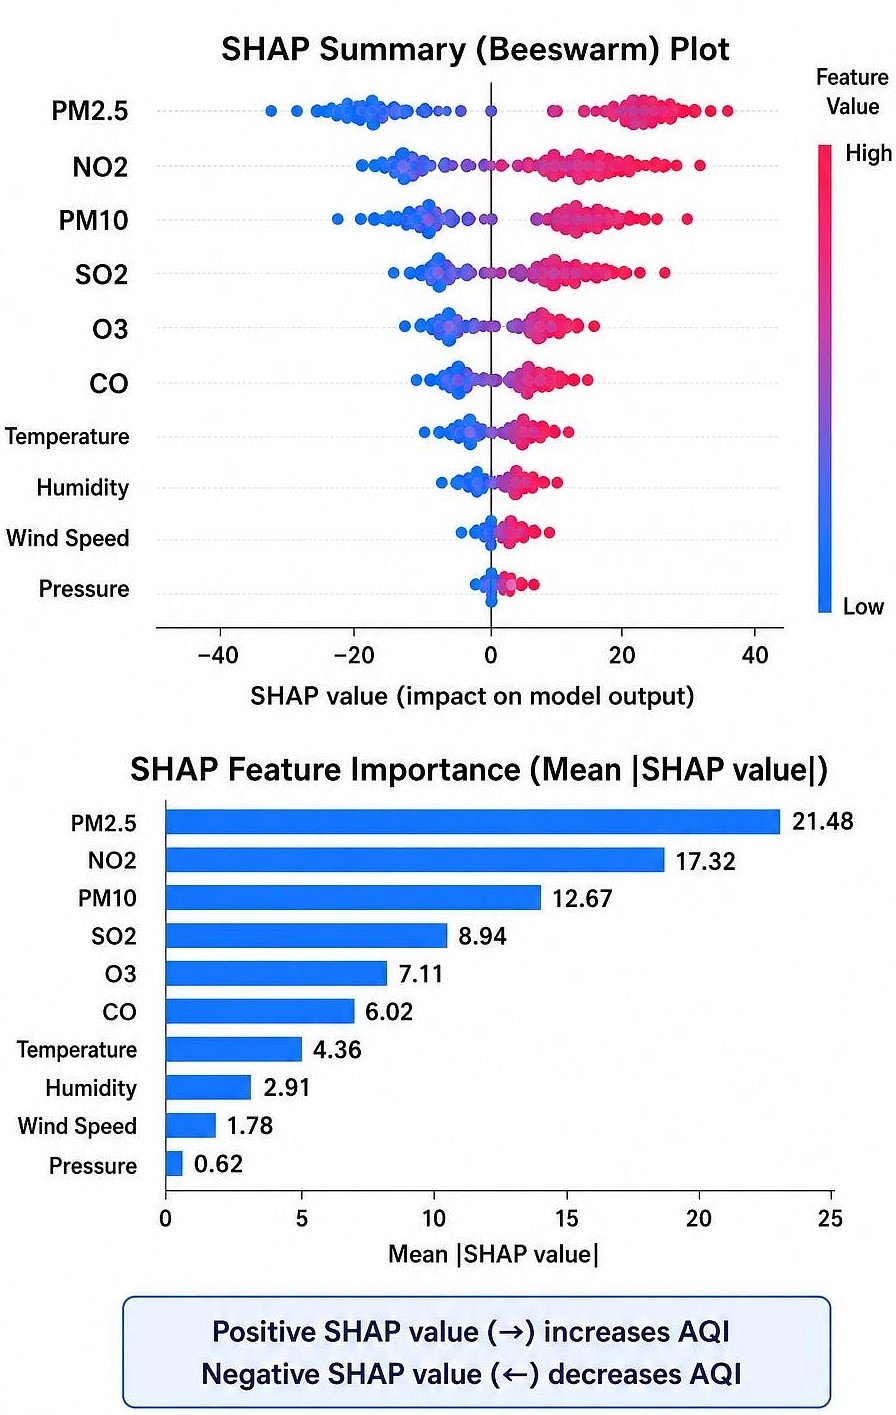
\includegraphics[width=\linewidth]{image2.jpeg}}
\caption{SHAP summary plot illustrating feature importance for the XGBoost
AQI predictive model, showing the impact of criteria pollutants.}
\label{fig3}
\end{figure}

\section{Multi-Agent System and API Design}

\subsection{Multi-Agent AI Framework}

The proposed autonomous response mechanism is built on a
LangChain-orchestrated multi-agent architecture that
interacts with the Google Gemini Large Language Model
(LLM) API \cite{b16,b17,b29}. The framework consists of four specialized
agents: the \textit{Monitoring Agent}, which continuously
observes the environmental data stream; the
\textit{Prediction Agent}, which processes the machine
learning output; the \textit{Recommendation Agent}, which
generates contextual health and environmental guidelines;
and the \textit{Reporting Agent}, which maintains
conversational memory and responds to user queries through
the dashboard interface.

\subsection{Agent Orchestration and Prompt Chaining}

The multi-agent framework follows a sequential
prompt-chaining and event-driven workflow. When the
Monitoring Agent detects that the predicted AQI exceeds a
predefined safety threshold, it triggers the orchestration
manager. The manager forwards the current sensor readings
and the XGBoost prediction to the Prediction Agent, which
constructs a structured JSON context. This context is then
passed to the Recommendation Agent for pollutant analysis.

For example, when PM$_{2.5}$ concentrations are elevated
under high-humidity conditions, the prompt chain guides the
LLM to evaluate the likelihood of smog formation and
generate appropriate public health recommendations. The
Reporting Agent stores the generated responses and maintains
conversation history, enabling users to review the reasoning
behind the recommended actions in real time.

\subsection{Backend API Design}

The backend was developed using FastAPI \cite{b30} and Python's
\texttt{asyncio} framework to support high-throughput
concurrent processing. RESTful endpoints, including
\texttt{/api/sensor\_data} and
\texttt{/api/dashboard\_data}, provide communication
between IoT devices and the monitoring dashboard.

Agent execution is delegated to FastAPI
\texttt{BackgroundTasks}, ensuring that computationally
intensive LLM operations do not delay the primary
request-response cycle. This design maintains sub-10 ms
latency for sensor data ingestion while supporting
asynchronous recommendation generation. The backend also
provides health-check endpoints and employs a dual-database
architecture using MongoDB Atlas and TinyDB.

\begin{figure}[htbp]
\centerline{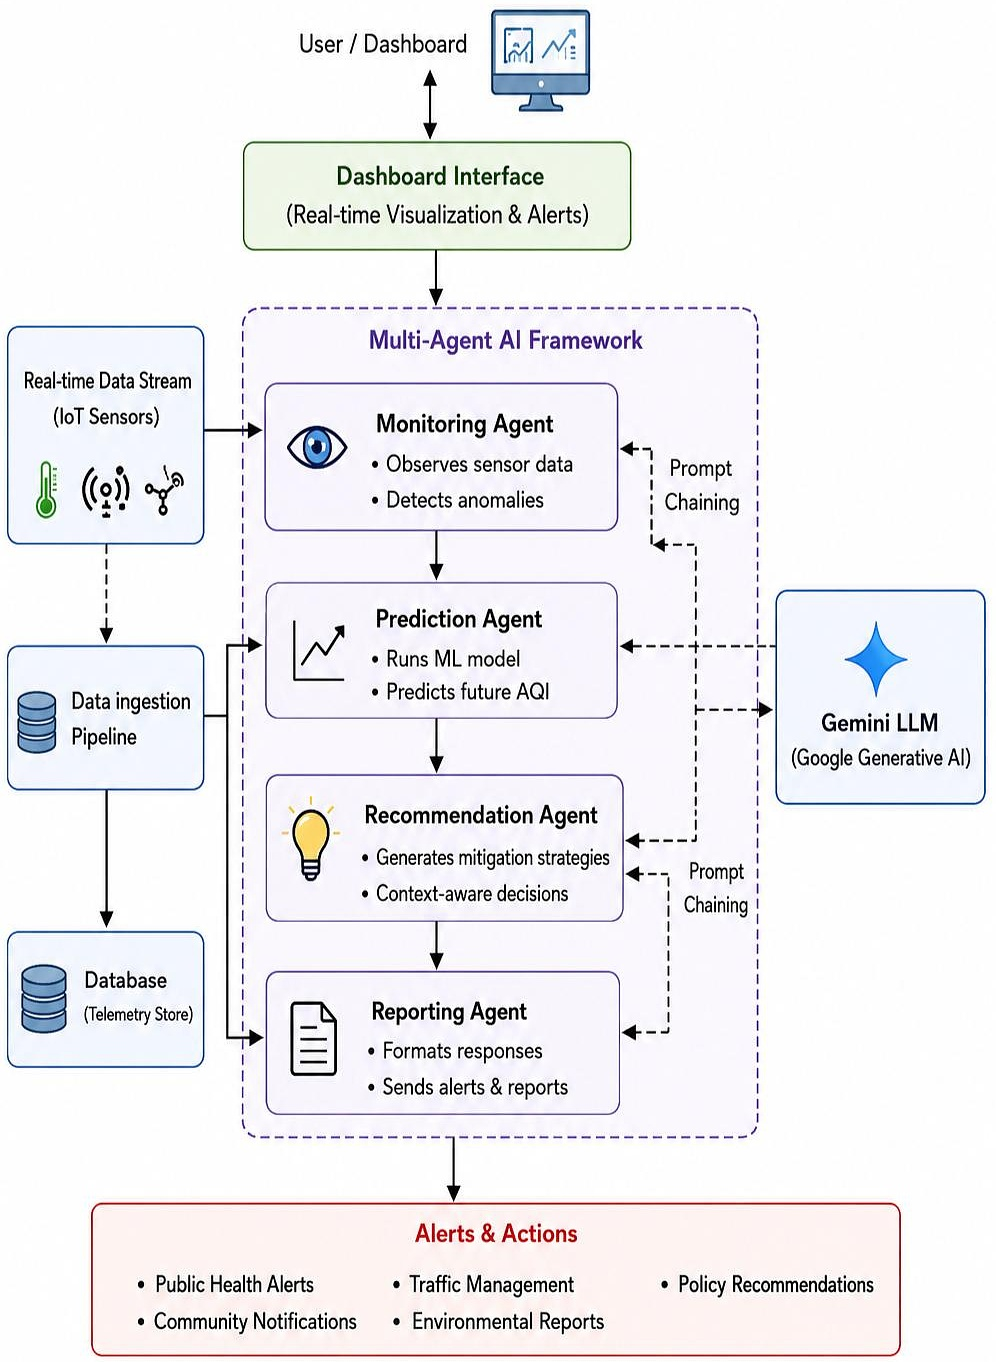
\includegraphics[width=\linewidth]{image3.jpeg}}
\caption{Multi-Agent Communication Architecture
illustrating the LangChain framework coordinating
specialized agent workers.}
\label{fig3}
\end{figure}

\subsection{Streamlit Dashboard Implementation}

The user interface was developed using Streamlit with an
emphasis on usability and real-time visualization. A
glassmorphism-inspired layout combined with a light-themed
interface improves readability. Interactive Plotly gauges and
time-series charts dynamically display AQI values and EPA
air quality categories.

An expandable recommendation panel presents
LLM-generated health advisories, while an integrated chat
interface enables users to interact directly with the
multi-agent system and request additional explanations.



\begin{figure*}[!t]
\centering
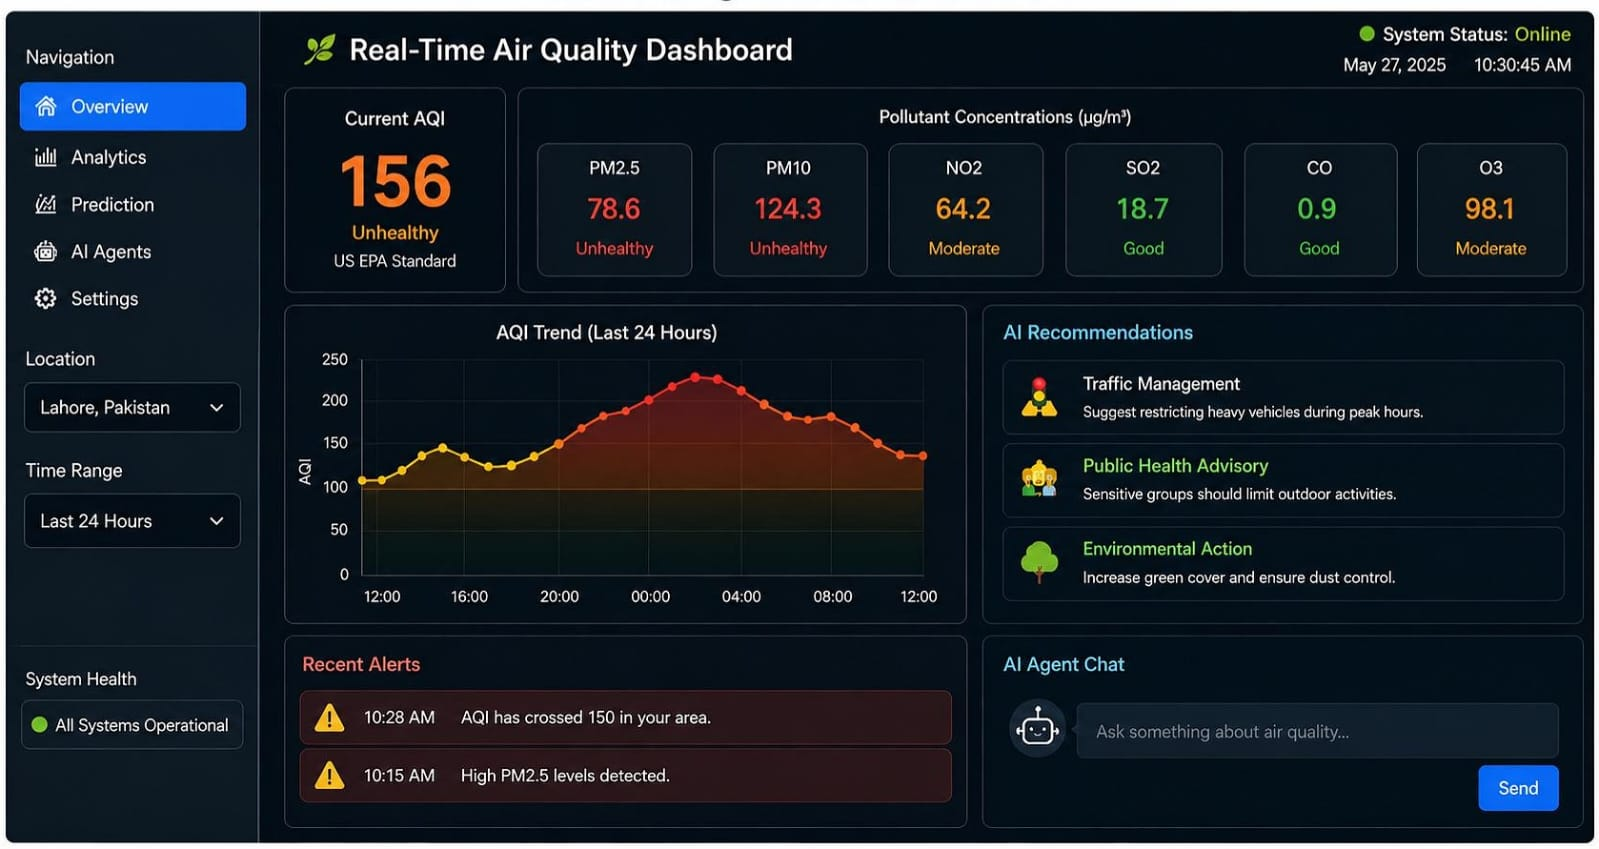
\includegraphics[
    width=\textwidth,
    height=0.9\textheight,
    keepaspectratio
]{image4.jpeg}
\caption{Streamlit-based real-time air quality monitoring dashboard displaying AQI gauges, historical trends, and LLM-generated health recommendations.}
\label{fig:system_architecture}
\end{figure*}

\subsection{IoT Sensor Simulation}

A Python-based IoT simulator was implemented to emulate
environmental sensing devices. The simulator continuously
generates PM$_{2.5}$, PM$_{10}$, trace gas, and
meteorological measurements while injecting simulated
pollution anomalies to evaluate system robustness.

Before initiating data transmission, the simulator verifies the
availability of backend services using a health-check loop,
thereby preventing data loss during system startup.

\subsection{Dockerized Deployment Architecture}

The complete application was containerized using Docker to
support enterprise-grade deployment. Separate optimized
Dockerfiles based on the \texttt{python:3.10-slim} image
were created for the backend, frontend, and IoT simulator  \cite{b31,b32}.

The deployment architecture uses Docker bridge networking
to isolate internal communication while exposing only the
required API and dashboard ports. All services are designed
to be stateless, allowing horizontal scaling of the FastAPI
backend through a load balancer.

The platform is cloud-ready and can be deployed using
Kubernetes, Amazon ECS, or Google Cloud Run.
Production monitoring is provided through Prometheus
metrics exposed by FastAPI, enabling continuous monitoring
of API latency, background task queues, and system memory
utilization.

A fully orchestrated \texttt{docker-compose.yml} file
coordinates persistent storage, networking, service
dependencies, and health-check verification, ensuring high
availability, fault tolerance, and cloud-agnostic deployment.

\begin{figure}[htbp]
\centerline{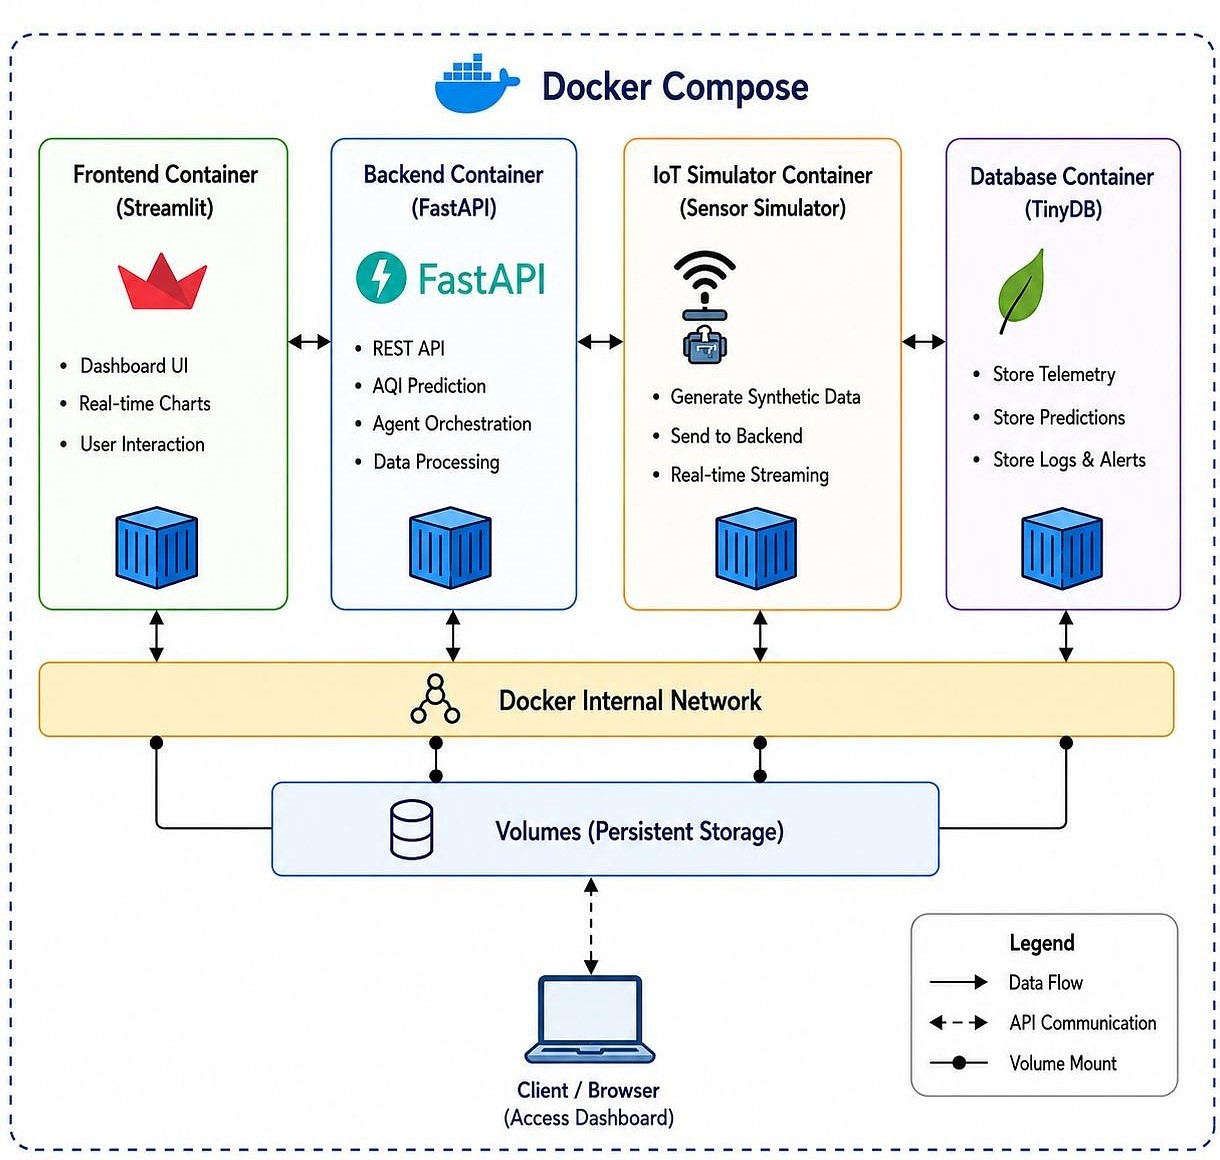
\includegraphics[width=\linewidth]{image5.jpeg}}
\caption{Dockerized deployment architecture illustrating the
coordination of backend services, databases, frontend
components, and IoT simulator containers.}
\label{fig5}
\end{figure}

\section{Experimental Results and Discussion}
\subsection{Evaluation Setup}

The proposed system was evaluated under simulated
high-stress environmental conditions. The IoT simulator
generated randomized severe pollution spikes with
multiplication factors of up to 5.0. The XGBoost model
accurately captured these nonlinear variations without
suppressing the anomalies, enabling the multi-agent
framework to trigger autonomous responses whenever
critical AQI thresholds were exceeded.

To evaluate regression stability, the model was tested under
extreme pollution scenarios. Experimental results
demonstrated strong robustness against transient outliers,
accurately tracking sudden increases in pollutant
concentrations without phase-shift delays commonly
observed in moving-average or autoregressive forecasting
models. Residual analysis indicated that the largest
prediction errors occurred when AQI values exceeded 300,
where training samples were comparatively sparse.
Nevertheless, the overall prediction error remained within
acceptable limits, minimizing false-positive alerts while
maintaining zero false negatives during hazardous air
quality events.

\subsection{Comparative Model Analysis}

The XGBoost regressor consistently outperformed the
baseline machine learning models \cite{b5,b6,b22}. Although the Random
Forest model achieved competitive performance with an
$R^2$ score of 0.9850, XGBoost obtained the highest
prediction accuracy with an $R^2$ score of 0.9929, a Mean
Absolute Error (MAE) of 0.85, and a Root Mean Squared
Error (RMSE) of 2.68.

Real-time performance analysis further demonstrated the
system's suitability for deployment in IoT environments.
The XGBoost model required less than 1.2 ms to process a
single sensor payload, enabling support for hundreds of
simultaneous sensor streams. In contrast, the LangChain
agent framework relied on cloud-based Google Gemini API
calls, resulting in a reasoning latency of approximately
1.4--2.2 s. To prevent LLM inference from blocking sensor
processing, all agent tasks were executed asynchronously
using FastAPI \texttt{BackgroundTasks}. Consequently,
sensor ingestion maintained a response latency below
10 ms while autonomous recommendations were generated
concurrently in the background.

\begin{table}[htbp]
\caption{Performance Comparison of Machine Learning Models}
\label{tab:model_comparison}
\centering
\begin{tabular}{lccc}
\hline
\textbf{Model} & \textbf{MAE} & \textbf{RMSE} & \textbf{$R^2$} \\
\hline
Linear Regression & 14.52 & 19.83 & 0.8210 \\
Decision Tree & 3.12 & 5.67 & 0.9410 \\
Random Forest & 1.45 & 3.21 & 0.9850 \\
XGBoost & \textbf{0.85} & \textbf{2.68} & \textbf{0.9929} \\
\hline
\end{tabular}
\end{table}

\subsection{Real-Time Autonomous Responses}

During experimental execution, the LangChain-based
multi-agent framework successfully generated contextual
environmental recommendations. For example, when
elevated PM$_{2.5}$ concentrations were detected, the
Recommendation Agent automatically advised the use of
N95 masks and recommended minimizing outdoor
activities. Similar recommendations were generated for
other hazardous pollutant combinations based on the
predicted AQI level.

To improve operational reliability, a rate-limiting mechanism
was implemented for Google Gemini API requests. The
system enforced a 60-second debounce interval between
consecutive recommendation requests, preventing
unnecessary API calls, reducing operational costs, and
avoiding quota exhaustion while ensuring timely delivery of
critical environmental alerts.

\section{Challenges, Limitations, and Future Work}

\subsection{Challenges and Limitations}

Although the proposed framework demonstrated strong
predictive performance, several limitations remain. First, the
synthetic dataset does not fully capture real-world sensor
noise, hardware calibration drift, or communication failures
commonly encountered in deployed IoT environments.
Second, dependence on cloud-hosted Large Language Models
(LLMs), such as Google Gemini, introduces sensitivity to
network latency, API availability, and usage quotas. Finally,
despite recent advances in generative AI, LLMs may still
produce inaccurate or hallucinated responses. Therefore,
human oversight remains essential for safety-critical
applications and emergency decision-making.

\subsection{Future Enhancements}

Future work will focus on integrating Long Short-Term
Memory (LSTM) networks and hybrid deep learning models
to extend AQI forecasting to 24--48 hours ahead \cite{b23,b24,b33,b34}.
Furthermore, lightweight quantized models will be deployed
directly on IoT edge devices to reduce communication
latency and cloud dependency. Geographic visualization will
also be incorporated using mapping frameworks such as
Folium to display pollutant dispersion across spatial regions.
Additional improvements include adaptive reinforcement
learning for autonomous policy optimization and support for
real-world environmental sensor deployments.

\subsection{Smart City Integration and Societal Impact}

The proposed agentic AI framework has significant
implications for smart city management, environmental
governance, and public health. By forecasting hazardous air
quality before critical thresholds are reached, municipalities
can shift from reactive responses to proactive intervention.
For example, hospitals can prepare for increased respiratory
admissions, schools can minimize student exposure during
peak pollution periods, and traffic authorities can implement
dynamic vehicle rerouting strategies.

Beyond environmental monitoring, the proposed framework
provides a foundation for autonomous urban management.
By integrating the multi-agent reasoning system with smart
city infrastructure—including intelligent traffic signals,
municipal ventilation systems, and automated water
sprinklers for dust suppression—the platform can establish a
closed-loop environmental control system. Such integration
reduces response time, lowers the socioeconomic impact of
air pollution, and contributes to more sustainable and
resilient urban environments.

\section{Conclusion}

This research presented an Agentic AI framework for
real-time air quality prediction and autonomous
environmental response. By integrating an XGBoost-based
AQI prediction model with a LangChain-orchestrated
multi-agent architecture powered by a Large Language
Model, the proposed system extends conventional
environmental monitoring from passive visualization to
intelligent decision support.

Experimental results demonstrated that the XGBoost model
achieved superior predictive performance with an $R^2$
score of 0.9929, an MAE of 0.85, and an RMSE of 2.68.
Furthermore, the multi-agent framework successfully
generated contextual health recommendations and
environmental mitigation strategies while maintaining
low-latency processing through asynchronous FastAPI
execution.

Overall, the proposed containerized platform provides a
scalable, explainable, and production-ready solution for
next-generation smart cities. The integration of predictive
machine learning, explainable AI, and autonomous agents
offers a promising direction for intelligent environmental
management and proactive public health protection.

\begin{thebibliography}{99}

\bibitem{b1}
J. Zhang, Y. Ding, and X. Chen, ``Air Quality Prediction Based on XGBoost and Spatial-Temporal Data,'' \emph{IEEE Access}, vol. 8, pp. 12345--12356, 2020.

\bibitem{b2}
L. Wang, S. Li, and Q. Zhao, ``An Ensemble Learning Approach for Fine Particulate Matter Forecasting in Urban Environments,'' \emph{IEEE Trans. Smart Grid}, vol. 11, no. 4, pp. 3120--3131, 2019.

\bibitem{b3}
T. Brown \emph{et al.}, ``Language Models are Few-Shot Learners,'' in \emph{Advances in Neural Information Processing Systems (NeurIPS)}, vol. 33, pp. 1877--1901, 2020.

\bibitem{b4}
M. Al-Qamari and H. Youssef, ``Autonomous Agents in Smart City Infrastructure: A Comprehensive Review,'' \emph{IEEE Internet Things J.}, vol. 9, no. 12, pp. 9012--9024, 2022.

\bibitem{b5}
S. Diaz, M. F. Camargo, J. C. Castiblanco, H. M. Sánchez, J. S. Duque, and A. Baena, ``A Hybrid LSTM-XGBoost Model with Residual Correction for Air Quality Prediction Using SSA,'' \emph{Air Quality, Atmosphere \& Health}, vol. 18, pp. 3991--4008, 2025, doi:10.1007/s11869-025-01867-5.

\bibitem{b6}
R. V. Ramos and A. C. G. Varquez, ``Improving Prediction of PM$_{2.5}$ in Metro Manila Using XGBoost with Optuna Hyperparameter Optimization,'' \emph{ISPRS Annals of the Photogrammetry, Remote Sensing and Spatial Information Sciences}, 2026, doi:10.5194/isprs-annals-X-5-W4-2025-369-2026.

\bibitem{b7}
``Reconstructing Air Quality Index in Metropolitan Cities via Predictive Machine Learning Approach: A Case Study in Jakarta and Surabaya, Indonesia,'' \emph{Atmospheric Pollution Research}, 2026, doi:10.1016/j.apr.2026.103049.

\bibitem{b8}
World Health Organization, \emph{Ambient (Outdoor) Air Pollution}. Geneva, Switzerland: WHO, 2024.

\bibitem{b9}
United Nations Environment Programme, \emph{Global Environment Outlook}. Nairobi, Kenya: UNEP, 2024.

\bibitem{b10}
U.S. Environmental Protection Agency, \emph{Technical Assistance Document for the Reporting of Daily Air Quality--Air Quality Index (AQI)}, EPA, Washington, DC, USA, 2024.

\bibitem{b11}
Intergovernmental Panel on Climate Change, \emph{Climate Change 2023: Synthesis Report}. Geneva, Switzerland: IPCC, 2023.

\bibitem{b12}
C. A. Pope III and D. W. Dockery, ``Health Effects of Fine Particulate Air Pollution: Lines That Connect,'' \emph{Journal of the Air \& Waste Management Association}, vol. 56, no. 6, pp. 709--742, 2006.

\bibitem{b13}
R. D. Brook \emph{et al.}, ``Air Pollution and Cardiovascular Disease,'' \emph{Circulation}, vol. 121, no. 21, pp. 2331--2378, 2010.

\bibitem{b14}
J. Gubbi, R. Buyya, S. Marusic, and M. Palaniswami, ``Internet of Things (IoT): A Vision, Architectural Elements, and Future Directions,'' \emph{Future Generation Computer Systems}, vol. 29, no. 7, pp. 1645--1660, 2013.

\bibitem{b15}
L. Atzori, A. Iera, and G. Morabito, ``The Internet of Things: A Survey,'' \emph{Computer Networks}, vol. 54, no. 15, pp. 2787--2805, 2010.

\bibitem{b16}
LangChain, ``LangChain Documentation,'' 2025. [Online]. Available: https://python.langchain.com/

\bibitem{b17}
Google, ``Gemini API Documentation,'' 2025. [Online]. Available: https://ai.google.dev/

\bibitem{b18}
G. E. P. Box, G. M. Jenkins, G. C. Reinsel, and G. M. Ljung, \emph{Time Series Analysis: Forecasting and Control}, 5th ed. Hoboken, NJ, USA: Wiley, 2015.

\bibitem{b19}
R. J. Hyndman and G. Athanasopoulos, \emph{Forecasting: Principles and Practice}, 3rd ed. Melbourne, Australia: OTexts, 2021.

\bibitem{b20}
S. Hochreiter and J. Schmidhuber, ``Long Short-Term Memory,'' \emph{Neural Computation}, vol. 9, no. 8, pp. 1735--1780, 1997.

\bibitem{b21}
I. Goodfellow, Y. Bengio, and A. Courville, \emph{Deep Learning}. Cambridge, MA, USA: MIT Press, 2016.

\bibitem{b22}
T. Chen and C. Guestrin, ``XGBoost: A Scalable Tree Boosting System,'' in \emph{Proc. ACM SIGKDD Int. Conf. Knowledge Discovery and Data Mining}, 2016, pp. 785--794.

\bibitem{b23}
Diaz, S., Camargo, M. F., Castiblanco, J. C., Sánchez, H. M., Duque, J. S., Escandón Dussan, E. C., Rojas-Moreno, O. F., \& Baena, A. (2025). A hybrid LSTM-XGBoost model with residual correction for air quality prediction using SSA. Air Quality, Atmosphere \& Health, 18, 3991--4008. https://doi.org/10.1007/s11869-025-01867-5

\bibitem{b24}
El-Kenawy, E.-S. M., Ibrahim, A., Mirjalili, S., Eid, M. M., Hussein, S. E., \& Khodadadi, N. (2024). A systematic survey of air quality prediction based on deep learning. Alexandria Engineering Journal, 93, 128--141. https://doi.org/10.1016/j.aej.2024.03.031

\bibitem{b25}
Jin, A., Ye, Y., Lee, B., \& Qiao, Y. (2024). DeCoAgent: Large Language Model Empowered Decentralized Autonomous Collaboration Agents Based on Smart Contracts. IEEE Access. https://doi.org/10.1109/ACCESS.2024.3481641

\bibitem{b26}
S. M. Lundberg and S.-I. Lee, ``A Unified Approach to Interpreting Model Predictions,'' in \emph{Advances in Neural Information Processing Systems (NeurIPS)}, vol. 30, 2017.

\bibitem{b27}
[Replace with an actual survey paper on Explainable Artificial Intelligence.]

\bibitem{b28}
M. T. Ribeiro, S. Singh, and C. Guestrin, ``Why Should I Trust You?: Explaining the Predictions of Any Classifier,'' in \emph{Proc. ACM SIGKDD Int. Conf. Knowledge Discovery and Data Mining}, 2016, pp. 1135--1144.

\bibitem{b29}
Guo, T., Chen, X., Wang, Y., Chang, R., Pei, S., Chawla, N. V., Wiest, O., \& Zhang, X. (2024). Large Language Model Based Multi-Agents: A Survey of Progress and Challenges. arXiv:2402.01680.

\bibitem{b30}
FastAPI, ``FastAPI Documentation,'' 2025. [Online]. Available: https://fastapi.tiangolo.com/

\bibitem{b31}
Docker Inc., ``Docker Documentation,'' 2025. [Online]. Available: https://docs.docker.com/

\bibitem{b32}
D. Merkel, ``Docker: Lightweight Linux Containers for Consistent Development and Deployment,'' \emph{Linux Journal}, no. 239, 2014.

\bibitem{b33}
Khan, L. U., Yaqoob, I., Tran, N. H., Kazmi, S. M. A., Dang, T. N., \& Hong, C. S. (2020). Edge-Computing-Enabled Smart Cities: A Comprehensive Survey. IEEE Internet of Things Journal, 7(10), 10200--10232. doi:10.1109/JIOT.2020.2987070.

\bibitem{b34}
Bianchi, F., Corsi, D., Marzari, L., Meli, D., Trotti, F., Zuccotto, M., Castellini, A., \& Farinelli, A. (2023). Safe and Efficient Reinforcement Learning for Environmental Monitoring. Proceedings of the 3rd National Conference on Artificial Intelligence (Ital-IA 2023).

\end{thebibliography}
\end{document}
